\documentclass[12pt]{article}

\newlength\tindent
\setlength{\tindent}{\parindent}
\setlength{\parindent}{0pt}
\renewcommand{\indent}{\hspace*{\tindent}}

%% packages
\usepackage{enumerate}
\usepackage{listings}
\usepackage{multicol}
\usepackage{amsmath}
\usepackage{caption}
\usepackage{subcaption}
\usepackage[a4paper,margin=2cm]{geometry}
% \usepackage[english, norsk]{babel}
\usepackage{fancyhdr}
\usepackage{pdfpages}
\usepackage{lastpage}
% \usepackage[demo]{graphicx}
\usepackage{graphicx}
\graphicspath{ {.} }


\date{}
\begin{document}

% intentionally empty
\author{Faculty of Mathematics and Natural Sciences}

\title{UNIVERSITY OF OSLO}

\maketitle 
\begin{center}
\textbf{Exam in GEO4300/9300 -- Geophysical Data Science}
\end{center}


Day of exam: 23 November, 2020 \\
Exam hours: 09:00 -- 12:00 (3 hours) \\ 

This examination paper consists of \pageref{LastPage} pages including this page. \\

Note: \\
1. This exam is an open book exam. All materials and tools are permitted.\\ 
2. There are in total 50 points in this exam.\\


\pagebreak

\section{Random variable parameter estimation}

A discrete random variable $X$ is defined by
  \begin{equation}
    X=
    \begin{cases}
      -1, & prob.=1/3 \\
       3, & prob.=1/2 \\
       4, & prob.=1/6
    \end{cases}
  \end{equation}

\begin{enumerate}[(a)] 
\item find the expected value
\item find the variance
\item find the mode
\item find the coefficient of variation
\end{enumerate}



\pagebreak
\section{Frequency analysis and linear regression}
\begin{enumerate}[(a)]
\item What is the probability to observe at least one 100-years flood or larger within a period of 10 years?
\item Figure 1A shows a simple linear regression between average runoff and median annual flood. Figure 1B shows the QQ-plot of the residual where the theoretical quantiles were calculated using the normal distribution. Describe which assumption of a simple linear regression is violated in this analysis, and discuss strategies that can be used to improve the analysis.
\end{enumerate}

\begin{figure}[h!]
    \centering
    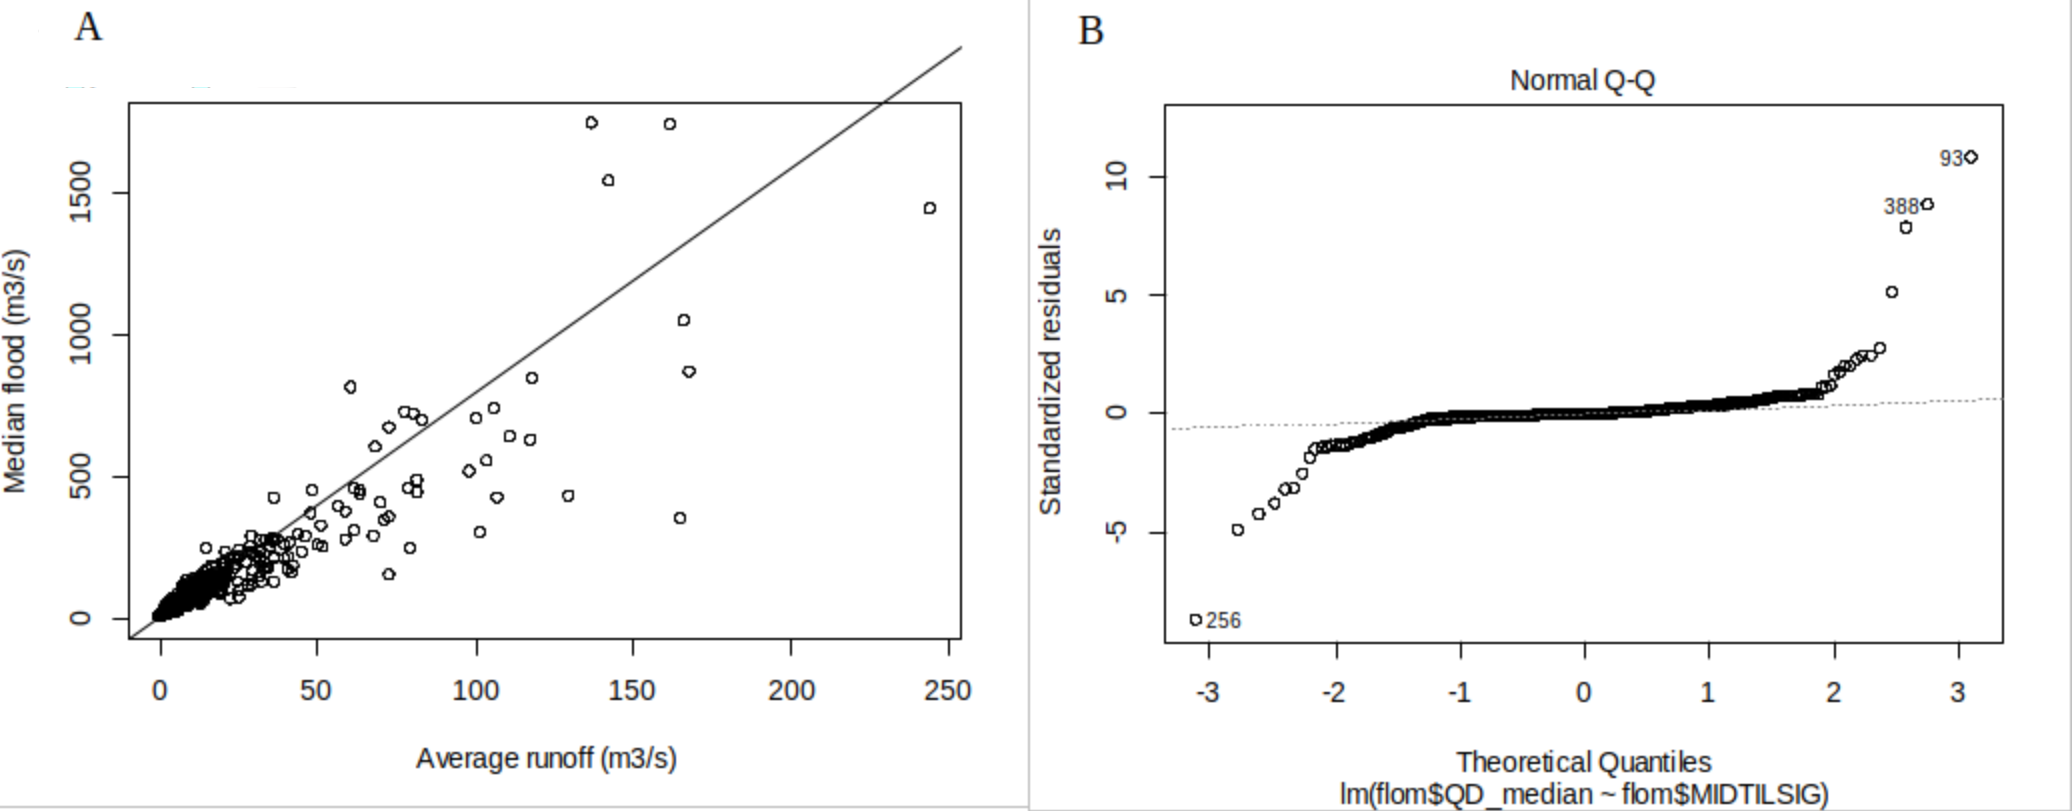
\includegraphics[width=.8\textwidth]{fig01} 
    \caption{A) linear regression, B) Q-Q plot.}
\end{figure}


\pagebreak
\section{Confidence intervals}
A sample of 30 random observations produced a mean of 145 and variance of 20. 
\begin{enumerate}[(a)] 
    \item What is the 95\% confidence interval on the mean assuming a normal distribution if 
    \begin{enumerate}[(i)] 
        \item the true variance is unknown and estimated as 20
        \item the true variance is 20
     \end{enumerate}
    \item What is the reason for the difference of results in part (i) and part (ii)?
    \item What is the 95\% confidence interval on the variance?
\end{enumerate}




\pagebreak

\section{Machine learning}
\begin{enumerate}[(a)] 
\item Why is it common to split the dataset into a training set and a test set when doing machine learning? In your answer, include in a relevant way the terms “training error” and “test error”
\item In many machine learning algorithms you have a parameter that controls the complexity of the model. Why do we want to control this complexity?
\end{enumerate}

\pagebreak

\section{Time series analysis and Fourier transformation}
Consider the following time series $X_t$ sampled once per second

\begin{figure}[h!]
    \centering
    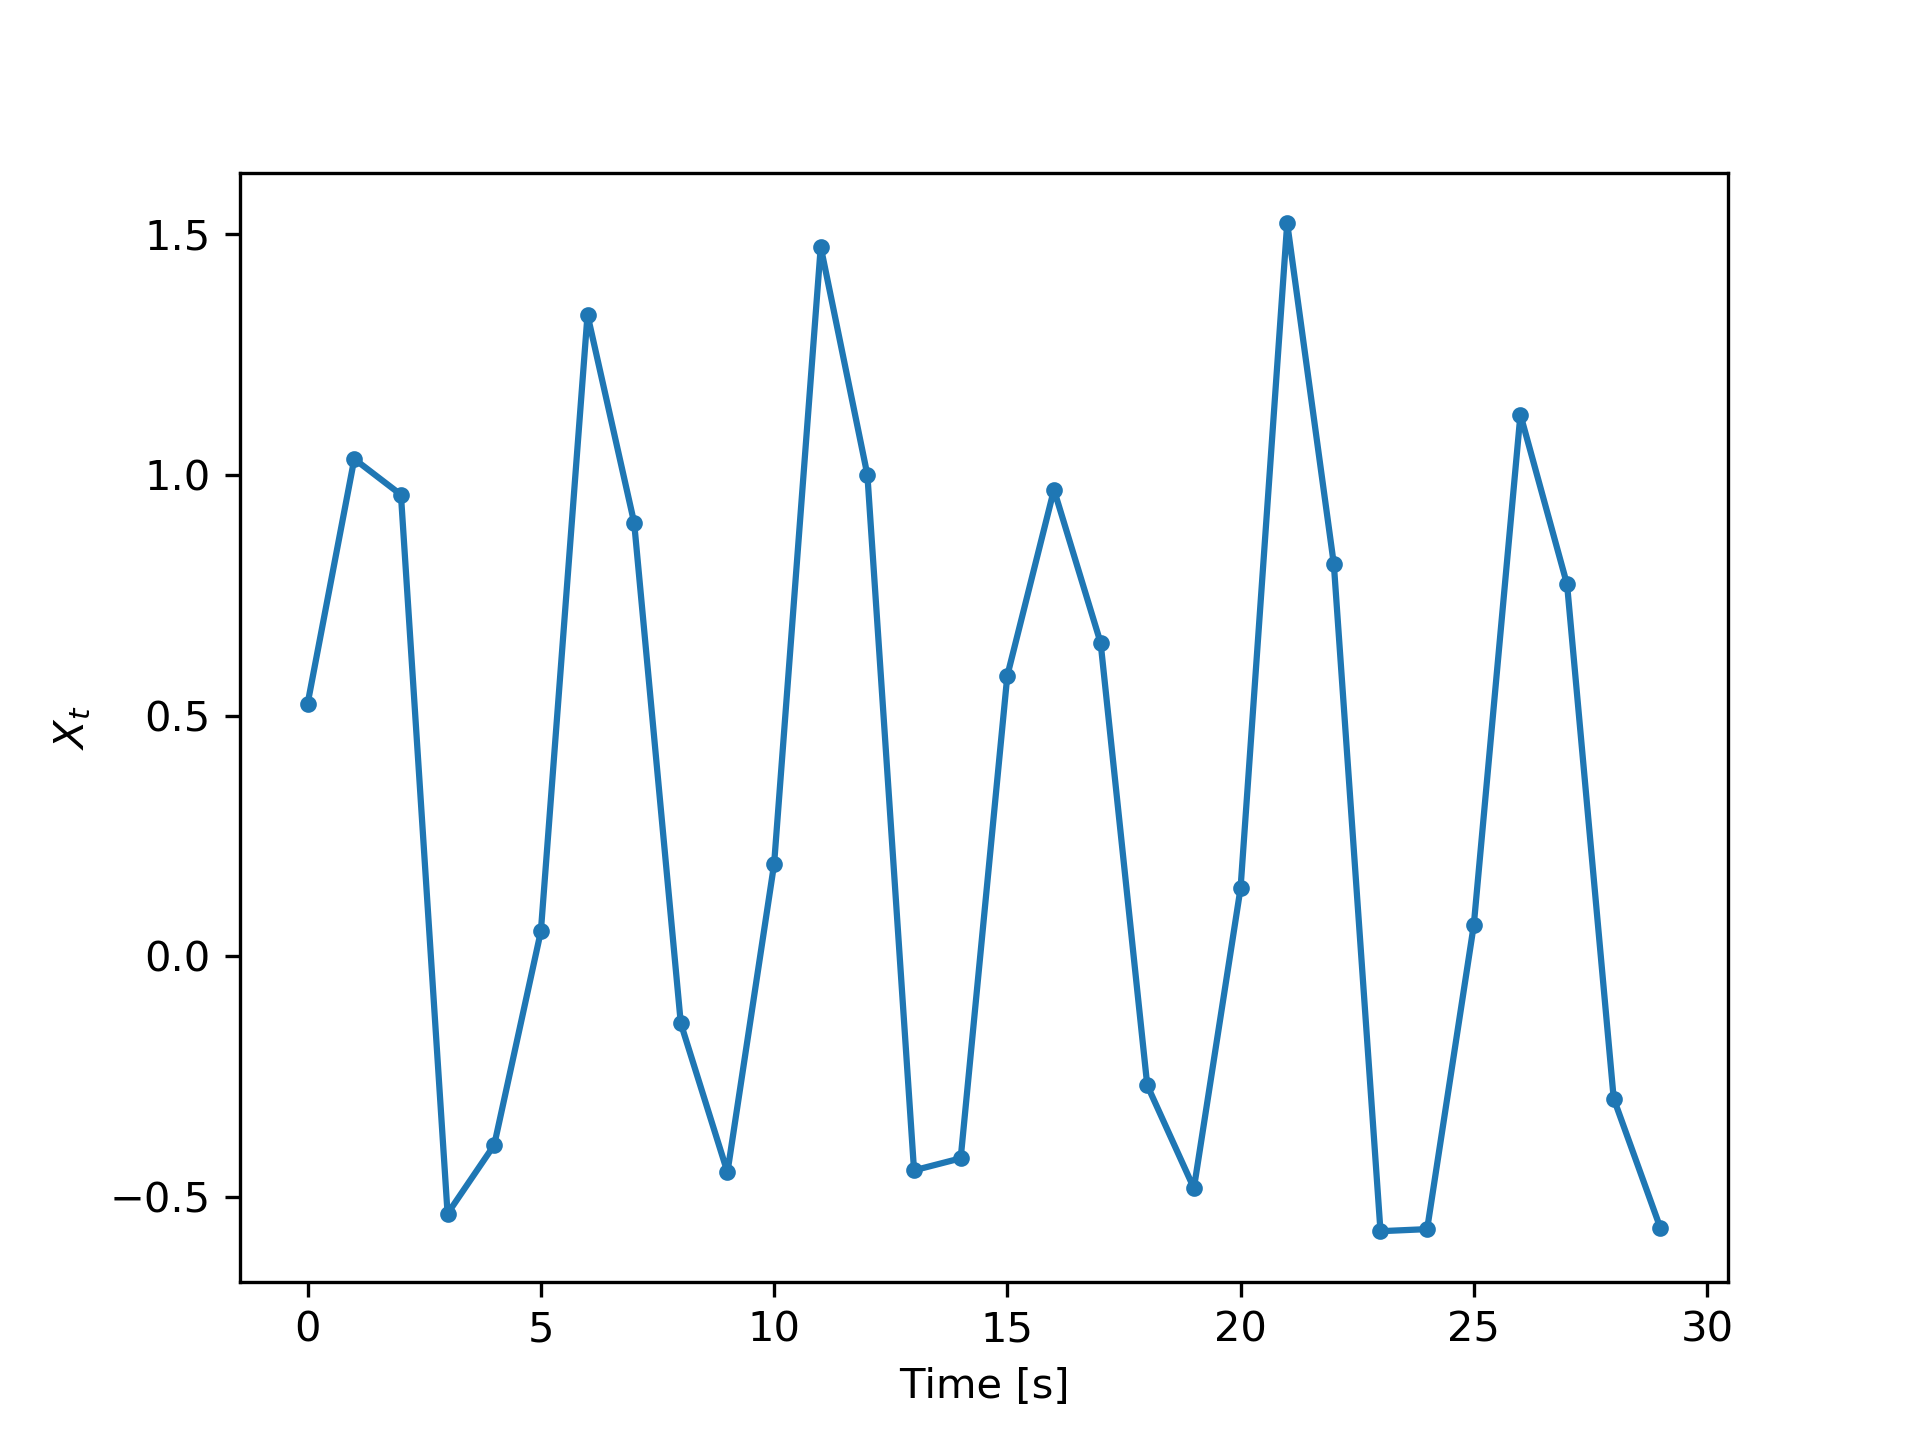
\includegraphics[width=.8\textwidth]{./fourier_figures/Fourier_ts} 
%    \caption{}
\end{figure}

\begin{enumerate}[(a)]
\item How could you test if there is a significant trend in $X_t$? Explain a suitable test.

\item The following three graphs show the absolute values for Fourier coefficients, defined as:
$$ X_k = \sum_{n=0}^{N-1} x_n \cdot e^{-i \, 2 \pi \, k \, n/N} $$

\begin{figure}[h!]
    \centering
    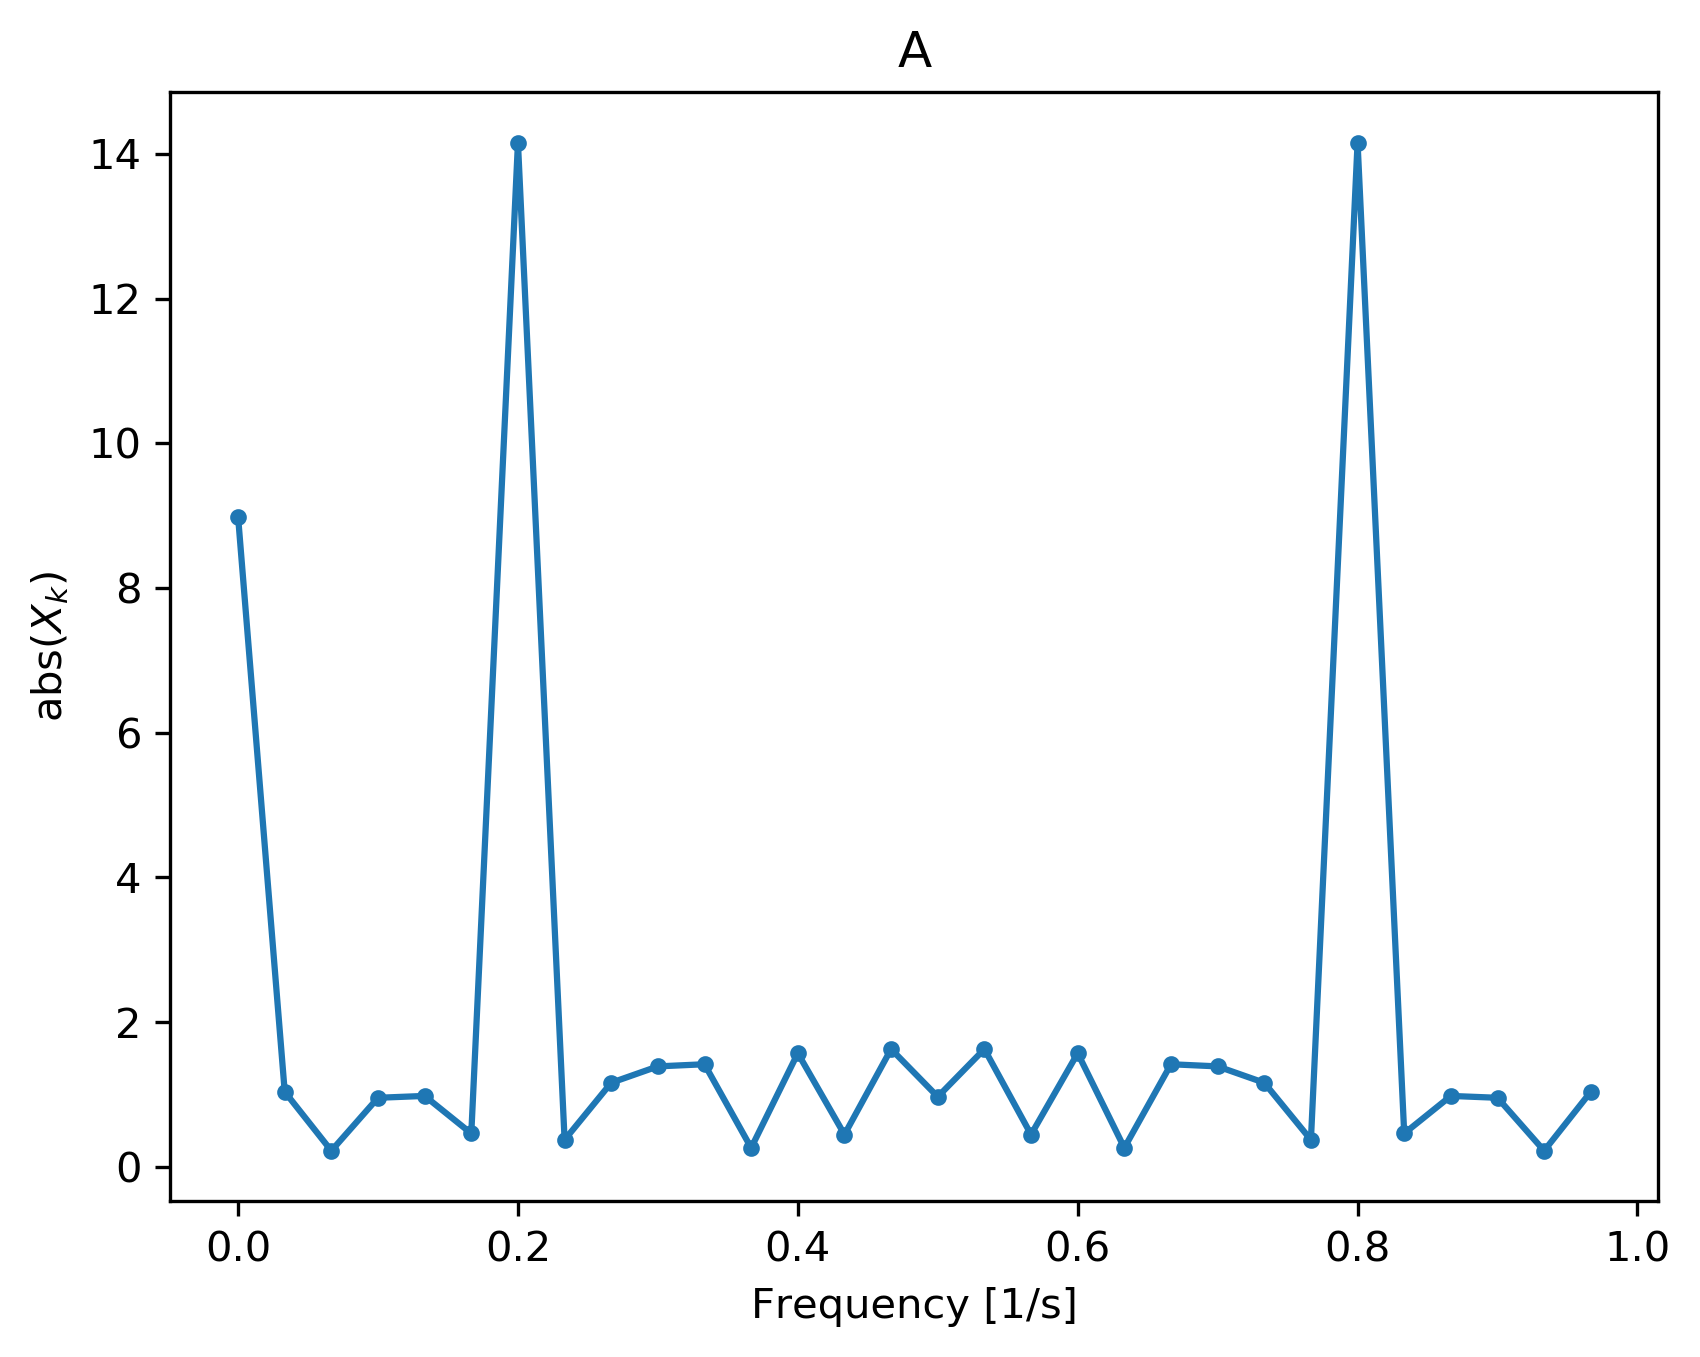
\includegraphics[width=.3\textwidth]{./fourier_figures/Fourier_A}
	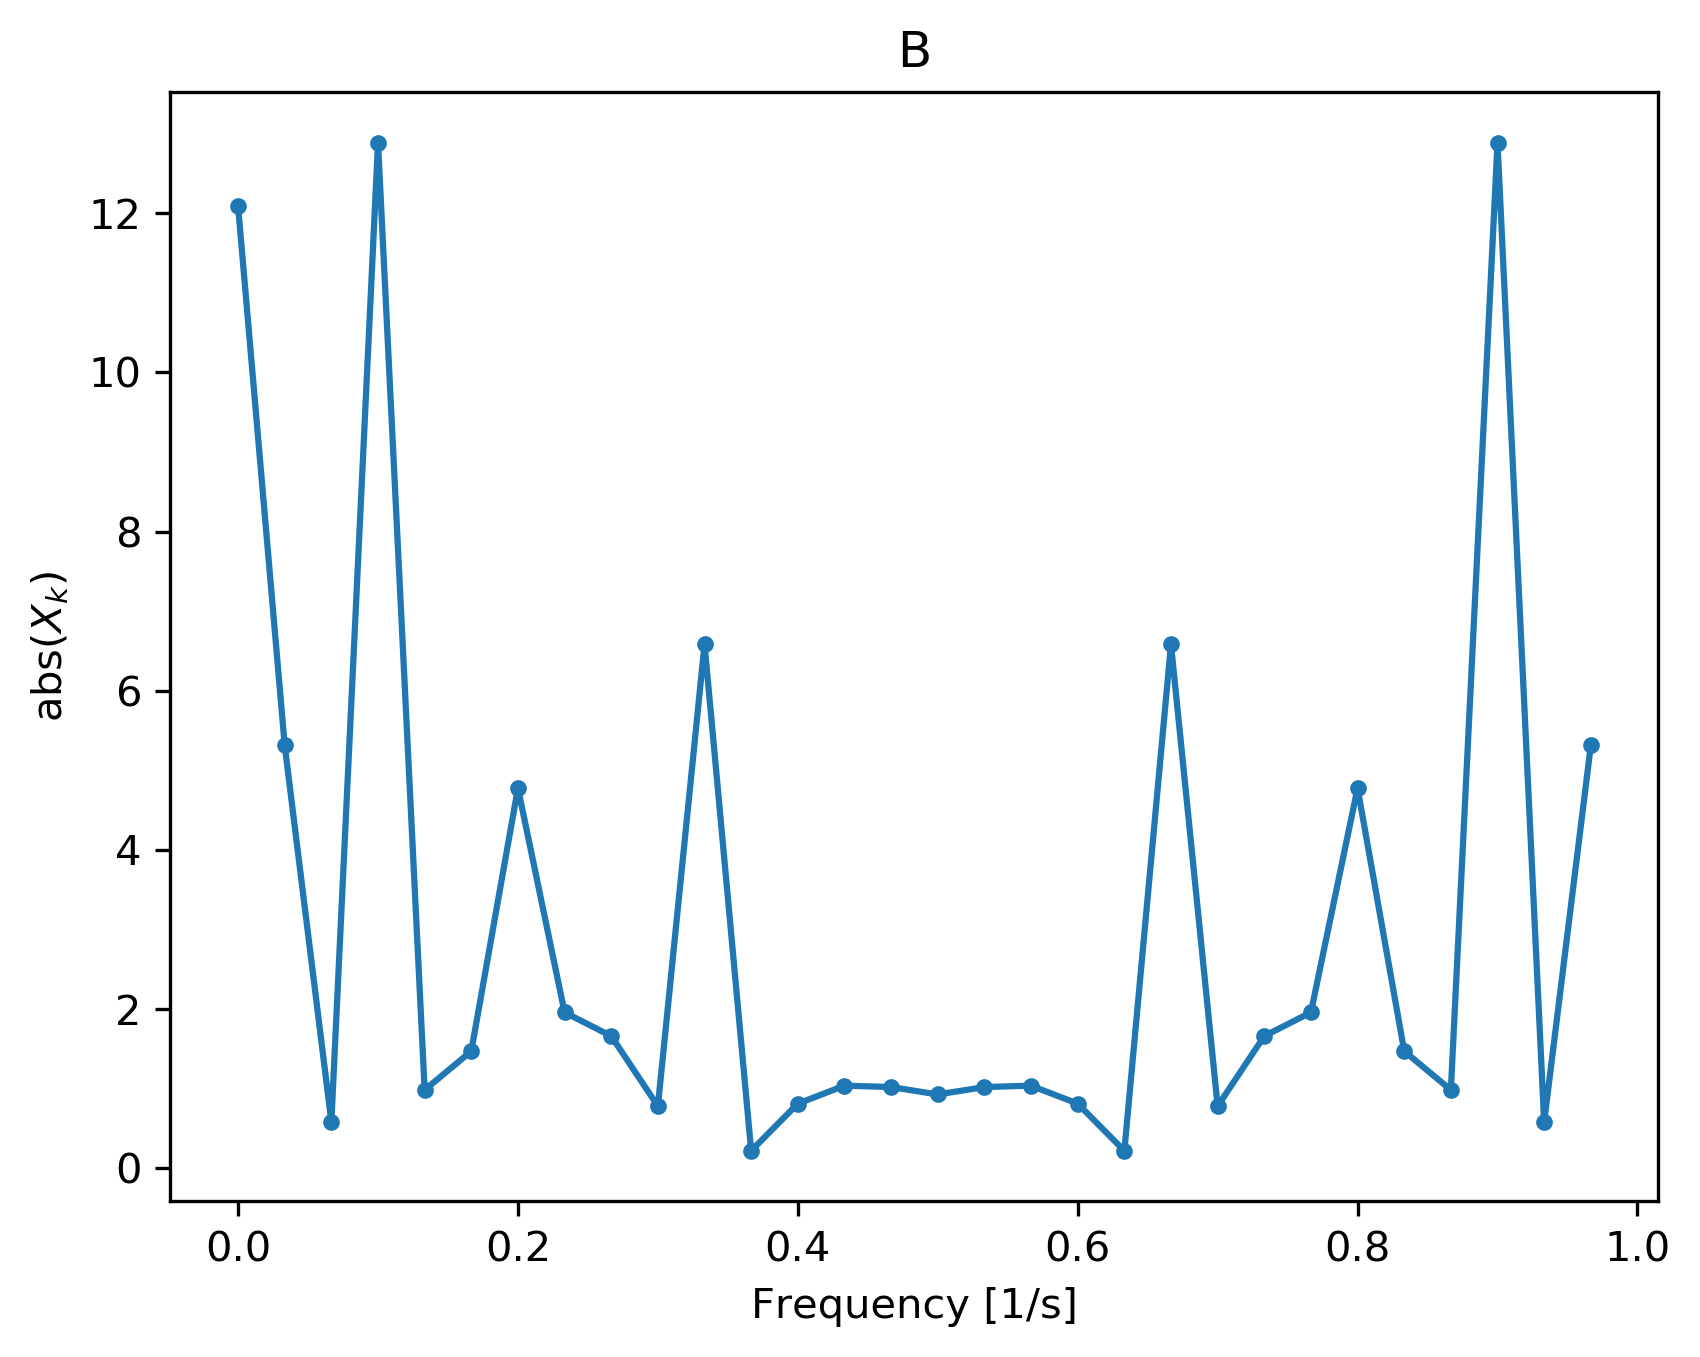
\includegraphics[width=.3\textwidth]{./fourier_figures/Fourier_B}
	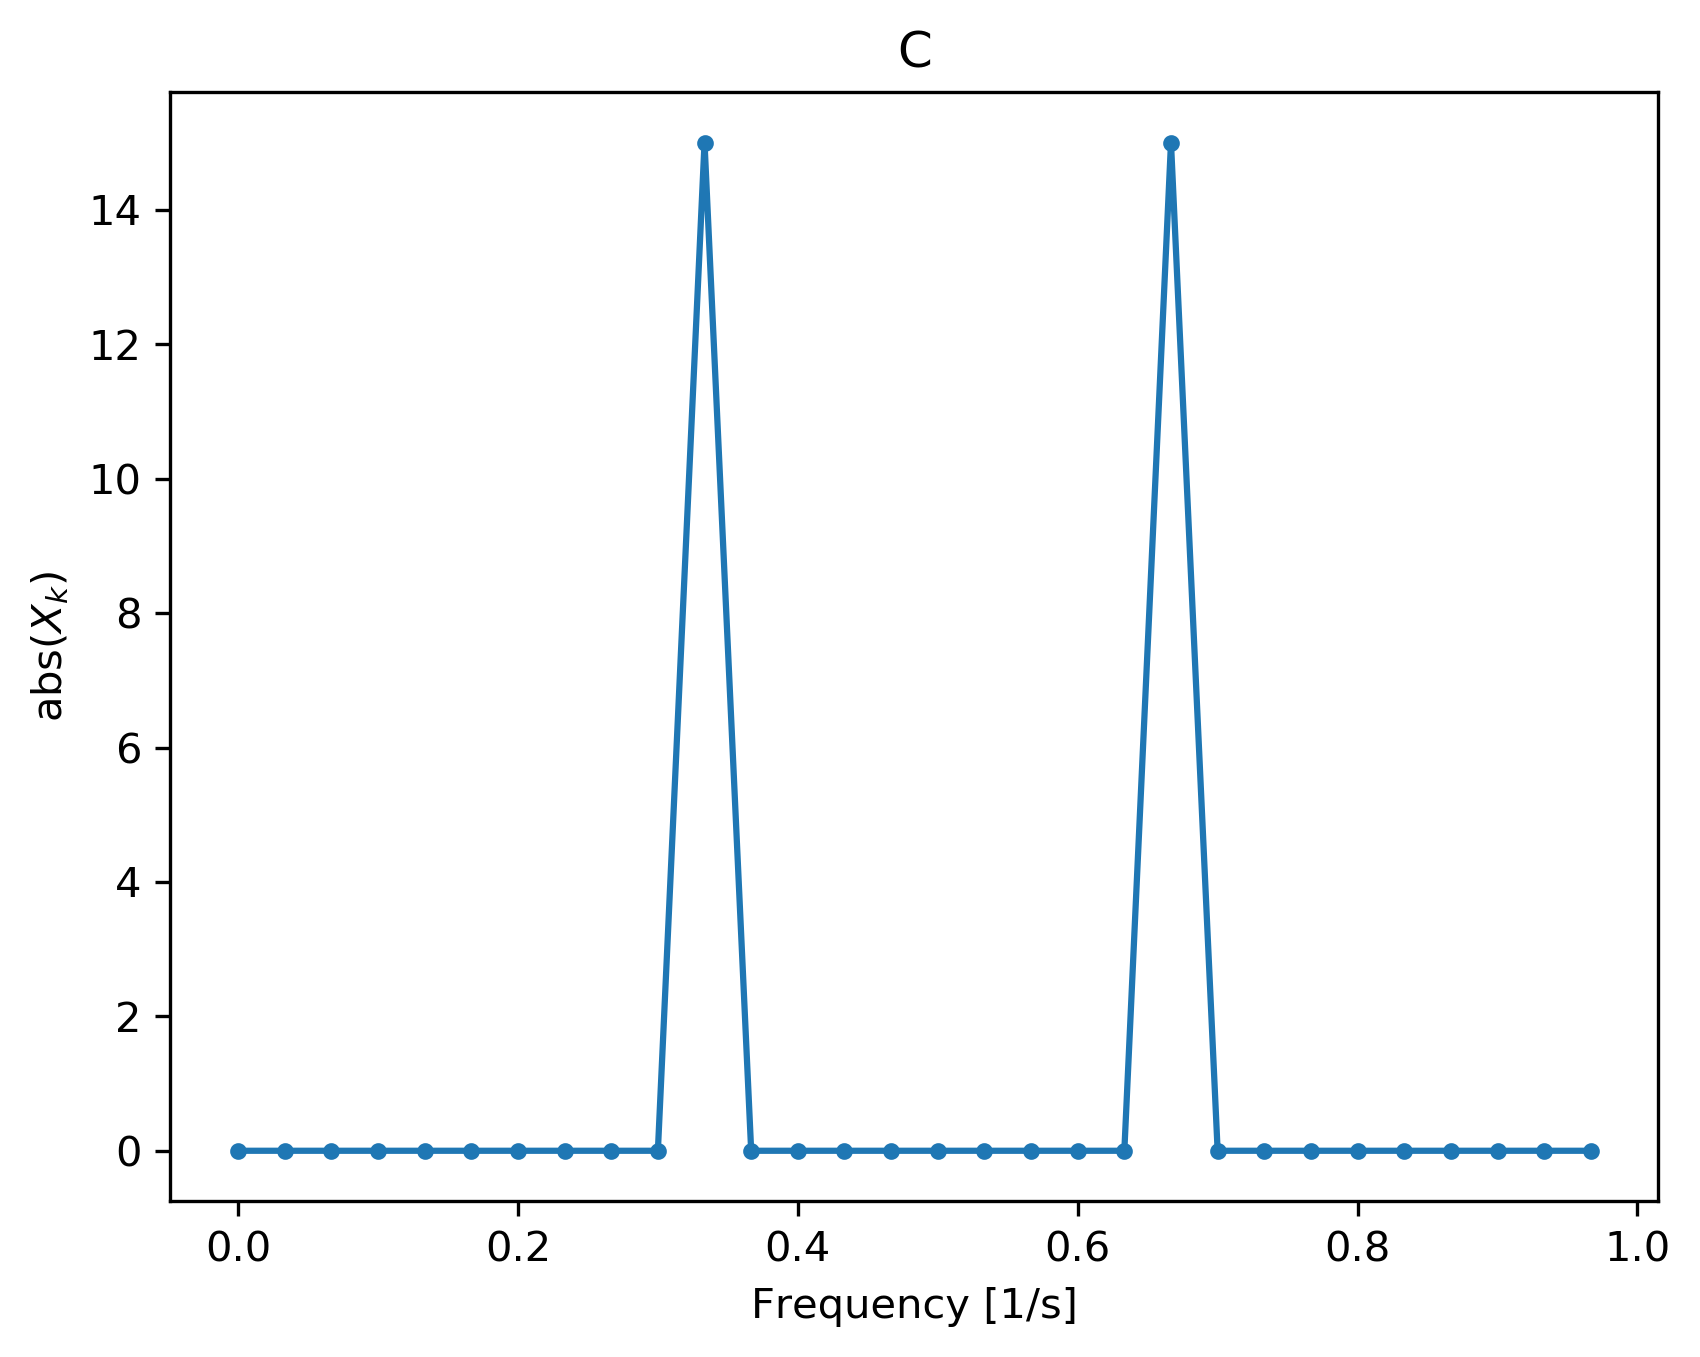
\includegraphics[width=.3\textwidth]{./fourier_figures/Fourier_C} 
%    \caption{}
\end{figure}
Which one of them (A, B or C) shows the Fourier transform of $X_t$? Explain your answer.


\end{enumerate}




%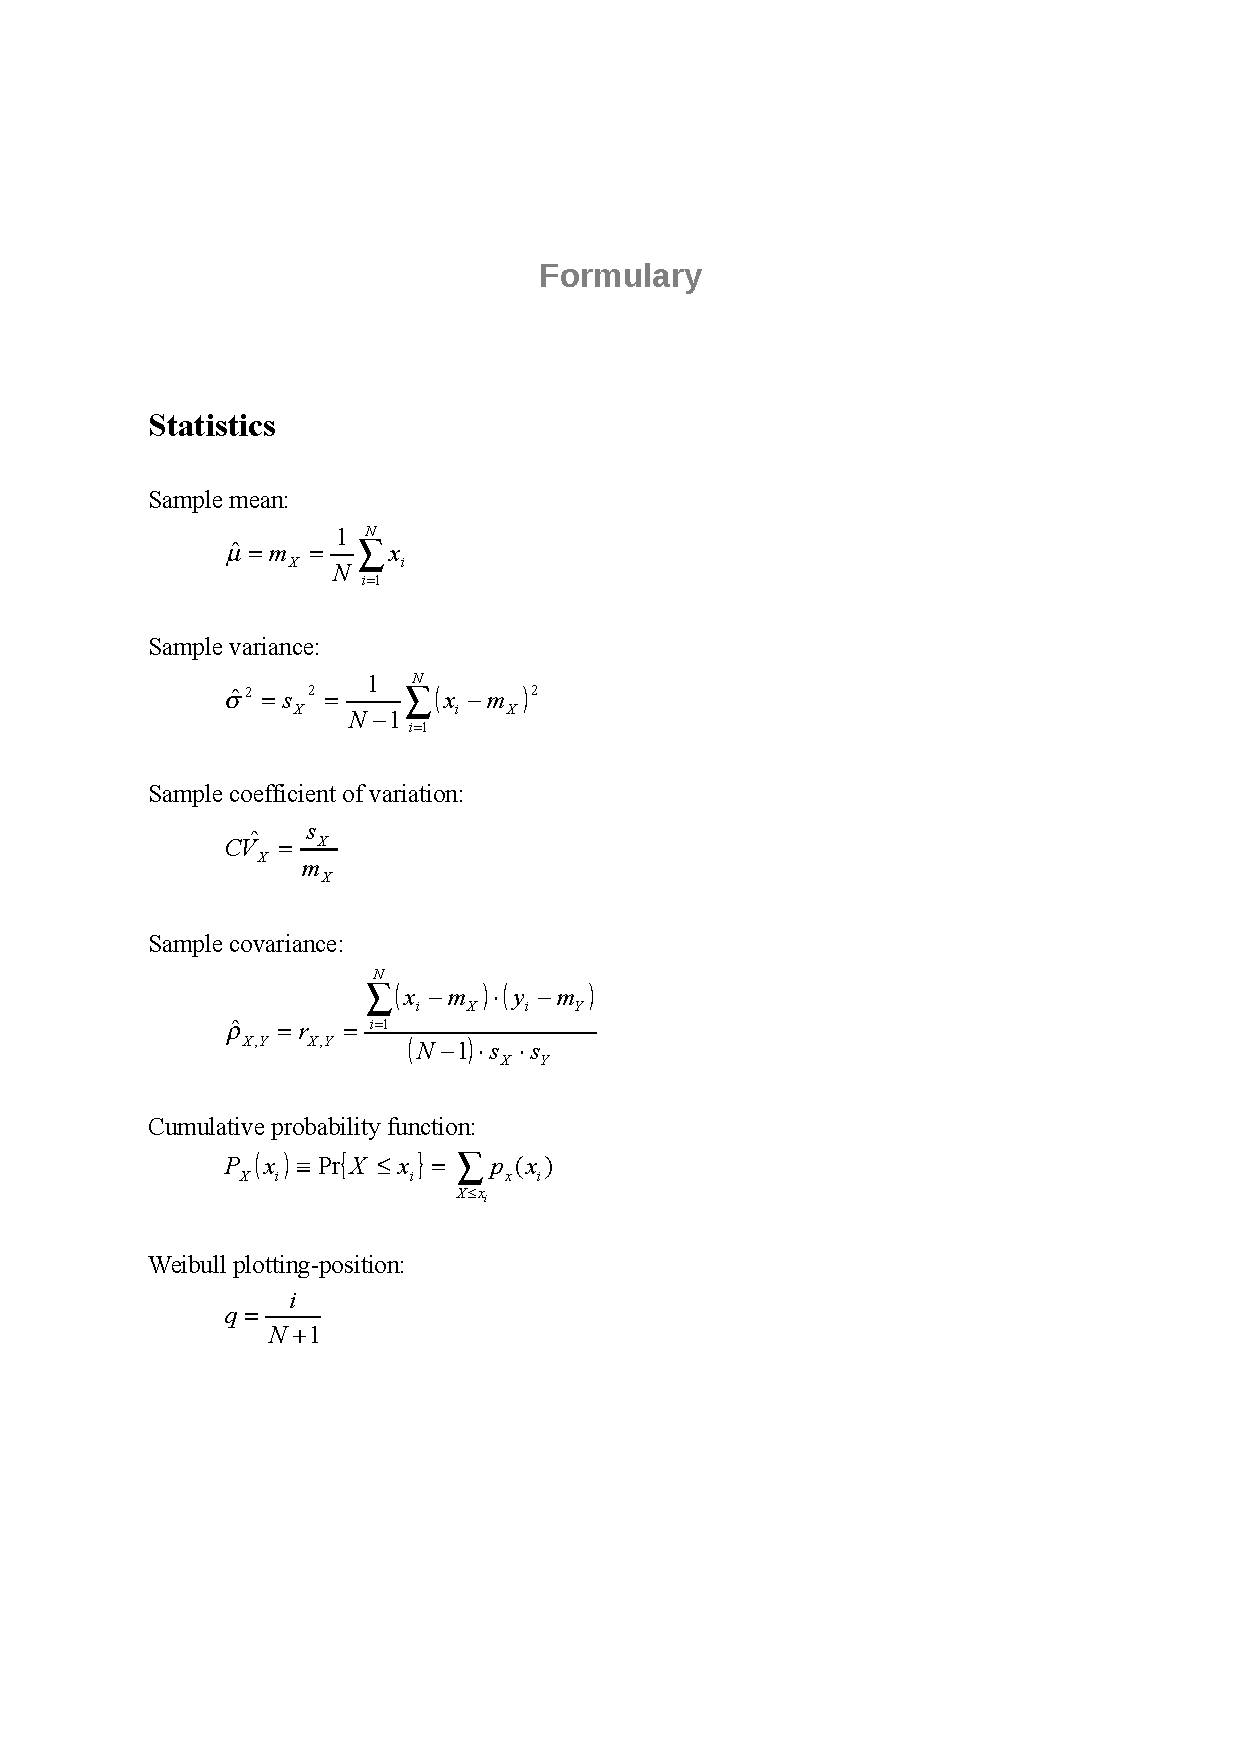
\includepdf[pages={1-12}]{formulary-2017_final.pdf}



\end{document}









